\documentclass[10pt]{article}

\usepackage{parskip}
\usepackage[margin=1in]{geometry} 
\usepackage{amsmath,amsthm,amssymb, graphicx, multicol, array}
\usepackage{makecell}
\usepackage{enumitem}
\usepackage{amssymb}
\usepackage{float}
\usepackage{href-ul}
 
\newcommand{\N}{\mathbb{N}}
\newcommand{\Z}{\mathbb{Z}}
 
\newenvironment{problem}[2][Problem]{\begin{trivlist}
\item[\hskip \labelsep {\bfseries #1}\hskip \labelsep {\bfseries #2.}]}{\end{trivlist}}

\begin{document}
 
\title{Multi-Objecive Optimization}
\author{Jakob Sverre Alexandersen\\
GRA4154 Supply Chain Optimization with Mathematical Programming\\
Lecture 10}
\maketitle

\tableofcontents
\newpage
\section{Intro}

\textbf{Why multi-objective?}

In reality, normally, there are more than one objective when making decisions: 
\begin{itemize}
    \item To minimize cost 
    \item To minimize completion time
    \item To minimize changes in the number of human resources 
    \item To maximize performance 
\end{itemize}
In many cases, these objectives are conflicting: 
\begin{itemize}
    \item When minimizing completion time, cost normally grows 
    \item When minimizing cost, performance/production/sales is normally sacrificed 
    \item \textbf{It is not possible to optimize all of them at the same time}
\end{itemize}
\section{MCDM, MADM and MODM}
\subsection{MCDM (multiple criteria decision making)}
\subsubsection{MODM (multiple objective DM)}
\begin{itemize}
    \item Normally continuous and uncountable set of alternatives/solutions 
    \item Aims to generate solutions 
\end{itemize}
\subsubsection{MADM (multiple attribute DM)}
\begin{itemize}
    \item Discrete and limited set of alternatives/solutions 
    \item Aims to rank existing alternatives/solutions 
\end{itemize}
\newpage 
\textbf{Selecting a MADM method}
\begin{figure}[H]
    \centering
    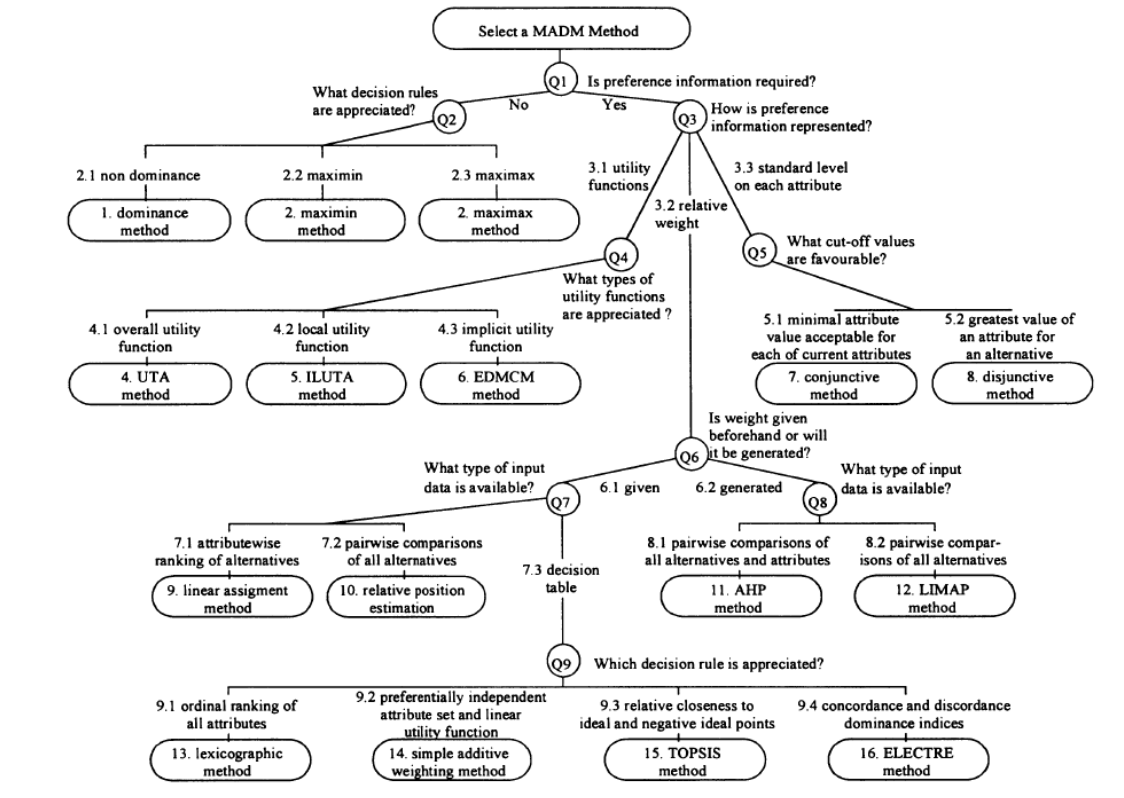
\includegraphics[width=0.8\textwidth]{2026-04-29-08-54-14.png}
\end{figure}
\subsection{What is a multi-objective optimization model?}
Same as a normal optimization model, but with multiple objectives 

\subsection{Which solution is the best?}
\begin{itemize}
    \item Decision variables: how much goods to be sent on each mode of transport: 
    \begin{itemize}
        \item Road 
        \item Rail 
    \end{itemize}
    \item Objectives: 
    \begin{itemize}
        \item Minimization of total cost 
        \item Minimization of average delivery time 
    \end{itemize}
\end{itemize}
\textbf{Setup:}

Imagine we have three alternatives within the region in the feasible solution set: 
\begin{itemize}
    \item A: Cost = 60, delivery time = 8
    \item B: Cost = 40, delivery time = 14
    \item C: Cost = 30, delivery time = 24
\end{itemize}
\newpage 
\subsection{Possible approach}
To merge multiple objectives into a single objective
\begin{itemize}
    \item Minimize Combined Objective (with delivery time measured in terms of customer dissatisfaction cost)
    \item Assume that in the example given on the previous page, Combined Objective is simply the sum of cost and delivery time 
\end{itemize}
If objectives are equally important, which solution is the best?
\begin{itemize}
    \item A: Combined Objective = 54
    \item B: Combined Objective = 54
    \item C: Combined Objective = 68
\end{itemize}
\textbf{Is it really that easy?}
\begin{itemize}
    \item Are all objectives equally important?
    \item If objectives are not equally important, how could one specify their relative imporance (weight)?
    \item The decision maker has to specify the relative importance of the objectives ``a priori'', i.e., in advance
    \begin{itemize}
        \item Is cost more important than delivery time?
        \item If yes, how much? Twice as important? 5 times as important?
    \end{itemize}
    \item This technique turns the multi-objective optimization problems into a single-objective one 
    \item This approach belongs to so-called ``preference-based procedures''
    \item It is called Weighted Sum Method 
\end{itemize}
\section{Weighted Sum Method}
\begin{itemize}
    \item The multi-objective model turns into a single-objective one as follows: 
    \begin{gather*}
        \min Z = \sum_{i = 1}^{m}w_if_i(x_1, x_2, \dots, x_n)\\
        \text{s.t.}\\
        g_1(x_1, x_2, \dots, x_n) \le b_1\\
        g_2(x_1, x_2, \dots, x_n) \le b_2\\
        \vdots \\
        g_k(x_1, x_2, \dots, x_n) \le b_k
    \end{gather*}
    \item The decision maker must specify the values of the weights $w_1, w_2, \dots, w_m $ in advance 
    \item Objectives must be normalized as well, i.e., must have the same scale 
    \item Weights can be determined by pairwise comparisons 
    \item By involving the decision maker in the process of optimization, weights can be changed interactively
\end{itemize}
\newpage 
\section{$\epsilon $-constrained method}
\begin{itemize}
    \item As in the weighted sum method, the multi-objective model turns into a single-objective one 
    \item One objective is chosen as the main objective to be optimized 
    \item Other objectives will appear in the model as constraints 
    \begin{itemize}
        \item In the case of minimization, a maximum acceptable level must be set for these objectives 
    \end{itemize}
    \begin{gather*}
        \min Z = f_\beta(x_1, x_2, \dots, x_n)\\
        \text{s.t.}\\
        f_i(x_1, x_2, \dots, x_n)\le \epsilon_i\quad\forall i = 1,\dots, m,\, i \neq \beta \\
        g_i(x_1, x_2, \dots, x_n)\le b_j\quad\forall j = 1,\dots, k
    \end{gather*}
    \item The decision maker must specify the values of the constraint limits $\epsilon_1, \dots, \epsilon_m $ in advance
    \item As in the weighted sum method, by involving the decision maker in the process of optimization, limits can be changed interactively
\end{itemize}
\subsection{Issues}
\begin{itemize}
    \item What if the objectives are not comparable?
    \item What if the decision maker does not know their relative importance in advance?
    \item What if one cannot set limits for the objectives?
    \item Which objective to be optimized and which ones should get turned into constraints?
    \item What if the decision maker wants to have different solutions in hand, observe the trade-offs between the objectives, and then decide which solution to choose?
    \item All of the aforementioned methods require higher-level and a-priori information
    \item If it is so easy to turn a multi-objective problem into a single-objective one, why should one go for multi objectives at all?
\end{itemize}
\newpage 
\section{Domination and Pareto Optimality}
\begin{itemize}
    \item If solution A is better than or equal to solution B in all of the objectives and strictly better than B in at least one objective, then solution A dominates solution B 
    \begin{itemize}
        \item Example: We want to buy a car, and the objectives are to minimize emissions and total cost ownership. The alternatives are a Skoda, Mercedes and a Tesla. Tesla has the lowest emissions, but is the most expensive as well. The Skoda is the cheapest, and has more emissions than the Tesla, but less than the Mercedes. 
        \item The Skoda dominates the Mercedes, while the Tesla cannot do the same. However, neither the Skoda nor the Tesla can dominate each other 
    \end{itemize}
    \item Given a set of $P $ solutions, the set $P'\subset P $ is called the Non-Dominated set, when $P' $ is the set of all solutions that cannot be dominated by any other solution in $P $
    \begin{itemize}
        \item The non-dominated set in the example above consists of the Skoda and the Tesla
    \end{itemize}
    \item \textbf{Pareto-Optimal set} is the set of feasible solutions which cannot be dominated by any other feasible solution. Each member of the Pareto-optimal set is called a \textbf{Pareto-optimal solution}
    \begin{itemize}
        \item In other words, Pareto-optimal set is $P' $, when $P $ is the set of all feasible solutions (feasible set)
    \end{itemize}
    \item So we are NOT talking about ONE optimal solution any longer 
    \item The weighted sum and $\epsilon $-constraint methods do not necessarily generate a Pareto-optimal solution
    \item These classical methods generate only one optimal solution. It would be good if we can generate all of the Pareto-optimal solutions, or at least a countable and finite set of uniformly distributed Pareto-optimal solutions. 
\end{itemize}
\subsection{Pareto-optimal and non-dominated fronts}
Mapping of Pareto-optimal and non-dominated sets into objective space: The figure on the right shows the Pareto-optimal front 
\begin{figure}[H]
    \centering
    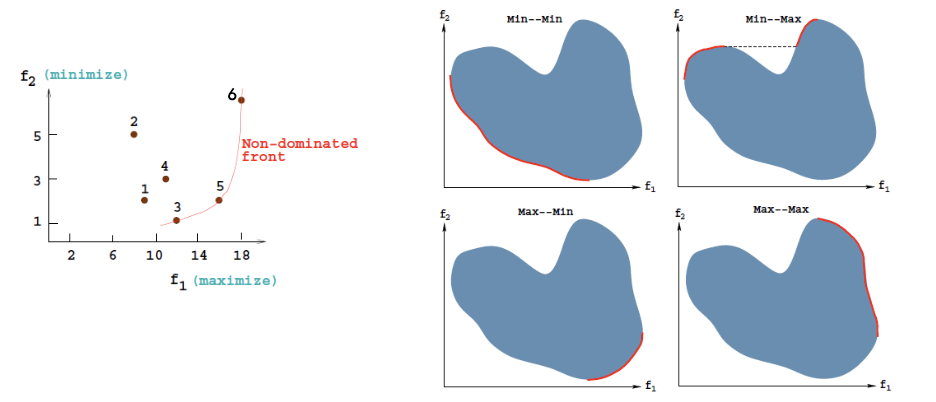
\includegraphics[width=0.8\textwidth]{2026-04-29-10-15-39.png}
\end{figure}
\newpage 
\subsection{Some Definitions}
\begin{itemize}
    \item If one optimizes the objectives separately and puts the optimal values of the objectives into a vector, that will be called \textbf{the ideal objective vector}
    \begin{itemize}
        \item If the objectives are conflicting, no feasible solution can generate all of the objective values in the ideal objective vector at the same time. Therefore, the ideal objective vector does not represent a feasible solution 
    \end{itemize}
    \item A vector of objective values whose elements are strictly better than the corresponding elements of the ideal objective vector (and therefore better than all of the feasible solutions), is called a \textbf{utopian objective vector}
    \begin{itemize}
        \item Some algorithms require a utopian objective vector to perform 
    \end{itemize}
    \item A vector of objective values whose elements are the worst values of the objectives observed in the Pareto-optimal set is called \textbf{the Nadir objective vector}
    \begin{itemize}
        \item The Nadir objective vector may or may not represent a feasible solution 
    \end{itemize}
\end{itemize}
\subsubsection{Ideal, Utopian and Nadir objective vectors}
\begin{figure}[H]
    \centering
    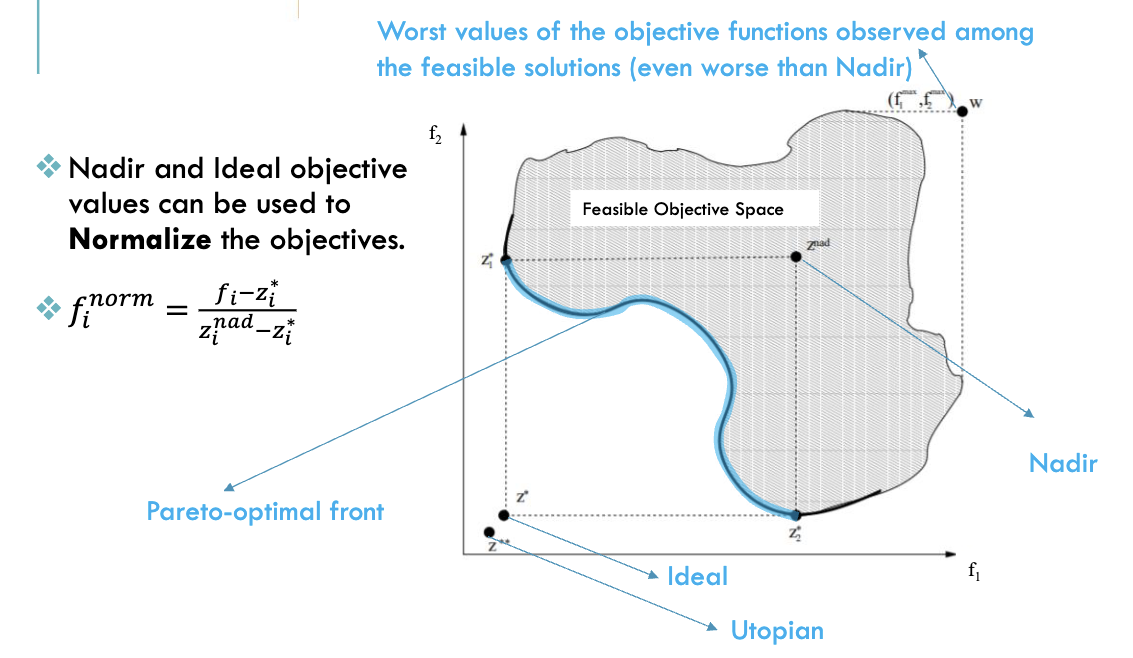
\includegraphics[width=0.8\textwidth]{2026-04-29-10-20-11.png}
\end{figure}
\newpage 
\section{Ideal multi-objective optimization}
\textbf{Process}
\begin{enumerate}
    \item Find a set of all Pareto-optimal solutions 
    \item Choose one solution from the set (higher-level information applied a-posteriori)
\end{enumerate}
\textbf{Challenges}
\begin{itemize}
    \item Converging to the Pareto-optimal front 
    \item Finding a diversely and evenly distributed set of Pareto-optimal solutions 
\end{itemize}
\section{A simple method to estimate Pareto-optimal front}
\textbf{Assume you have two objectives $f_1 $ and $f_2 $}
\begin{enumerate}
    \item Choose an objective, say $f_1 $, and determine its optimal value $V_1 $. For the same solution that gives you $V_1 $, find the value of $f_2 $ and denote it as $V_2 $. Then $(V_1, V_2) $ is a point on the Pareto-optimal front. 
    \item For values $V $ of $f_2 $ that are better than $V_2 $, solve the optimization problem in step 1 with the additional constraint that the value of $f_2 $ is at least as good as $V $. Varying $V $ (over values of $V $ preferred to $V_2 $) yields other points on the Pareto-optimal fron 
    \item Step 1 lovated one endpoint on the Pareto-optimal front. Now determine the best value of $f_2 $ that can be attained, to obtain the other endpoint of the Pareto-optimal fron 
\end{enumerate}
\subsection{General form of the previous algorithm}
\begin{itemize}
    \item Assume we know a classical optimization method to optimize a single-objective optimization problem $P $ with constraints $(\vec{X}\in S) $ and can find a near-optimum solution $\vec{x}^* $. Assume we want to find $K $ different efficient solutions 
    \item Step 1: Find individual optimum solutions $\vec{x}^{*i} $ for all objectives, where $i = 1, 2, \dots, M $
    \item Step 2: Choose $K $ points $\epsilon^{(k)} $ uniformly in the $(M - 1) $-dimensional plane having objectives $i = 1 $ to $i = M - 1 $ as coordinate directions 
    \item Step 3: Solve each subproblem $(k = 1, \dots, K) $ as follows:
    \begin{gather*}
        \min Z = f_M(\vec{x})\\
        \text{s.t.}\\
        f_i(\vec{x})\le \epsilon_i^{(k)},\quad\forall i \in \{1, 2, \dots, M - 1\} \\
        \vec{x}\in S
    \end{gather*}

    Call the optimal solution $\vec{x}^{*(k)} $ and corresponding objective vector $f^{*(k)} $
    \item Step 4: Declare the non-dominated set as the set of efficient sets: 
    \begin{gather*}
        F = \text{non-dominated} (f^{*(1)},\dots, f^{*(k)})
    \end{gather*}
\end{itemize}
\newpage 
\section{A simple linear multi-objective optimization example}
\begin{center}
    \begin{tabular}{|c|c|c|}
        \hline 
        \textbf{Cement} & \textbf{Type1} & \textbf{Type2} \\\hline 
        \textbf{Profit /ton (USD)} & 700 & 900\\\hline
        \textbf{CO2 emissions /ton (g)} & 2100 & 2900\\\hline
        \textbf{Mixer hrs /ton} & 3 & 4\\\hline
        \textbf{Soil /ton (tons)} & 1.5 & 1.2\\\hline
    \end{tabular}
\end{center}
\begin{center}
    \begin{tabular}{|c|c|}
        \hline 
        \textbf{Desirable profit /week (USD)} & 50,000 \\\hline 
        \textbf{Desirable CO2 emissions /week (g)} & 140,000 \\\hline 
        \textbf{Mixer hrs available /week} & 324 \\\hline 
        \textbf{Soil available /week (tons)} & 150 \\\hline 
    \end{tabular}
\end{center}
Let: 
\begin{itemize}
    \item $x_i $: Tons of cement type $i $ produced per week
\end{itemize}
\subsection{Version 1: profit maximization}
\begin{gather*}
    \max Z = 700x_1 + 900x_2\\
    \text{s.t.}\\
    3x_1 + 4x_2 \le 324\\
    1.5x_1 + 1.2x_2 \le 150\\
    x_i \ge 0 \quad\forall i \in \{1, 2\}
\end{gather*}
\subsection{Version 2: CO2 emissions minimization}
\begin{gather*}
    \min Z = 2100x_1 + 2900x_2 \\
    \text{s.t.}\\
    3x_1 + 4x_2 \le 324\\
    1.5x_1 + 1.2x_2 \le 150\\
    x_i \ge 0 \quad\forall i \in \{1, 2\}
\end{gather*}
\textbf{Solution space and objective space }
\begin{figure}[H]
    \centering
    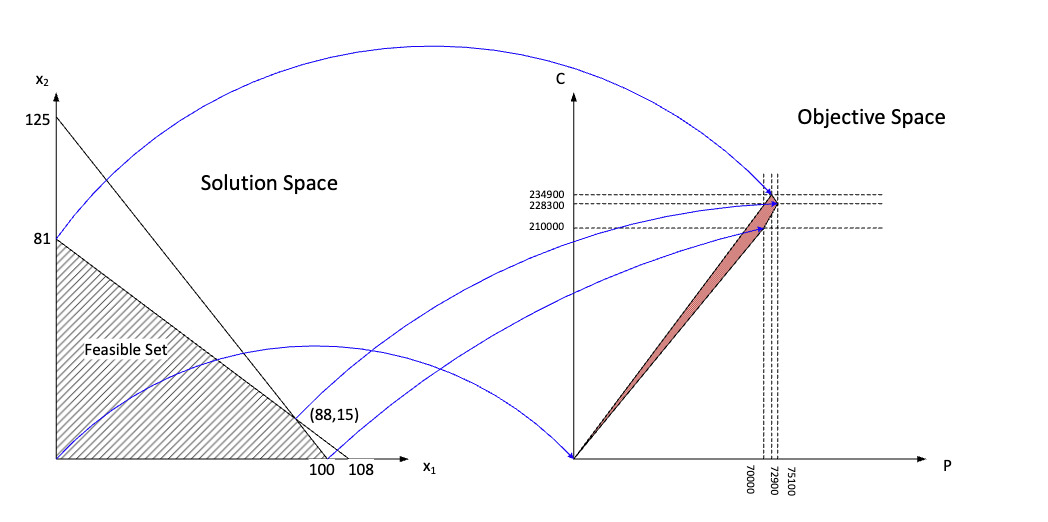
\includegraphics[width=0.8\textwidth]{2026-04-29-10-49-36.png}
\end{figure}
\newpage 
\textbf{Pareto-optimality}
\begin{figure}[H]
    \centering
    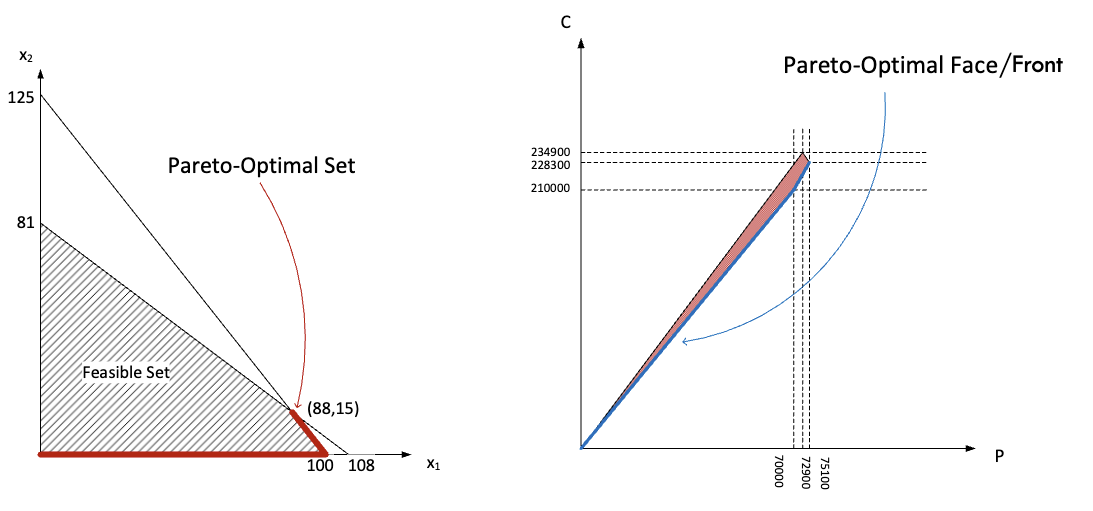
\includegraphics[width=0.8\textwidth]{2026-04-29-10-50-37.png}
\end{figure}
\textbf{Ideal, Utopian and Nadir solutions}
\begin{figure}[H]
    \centering
    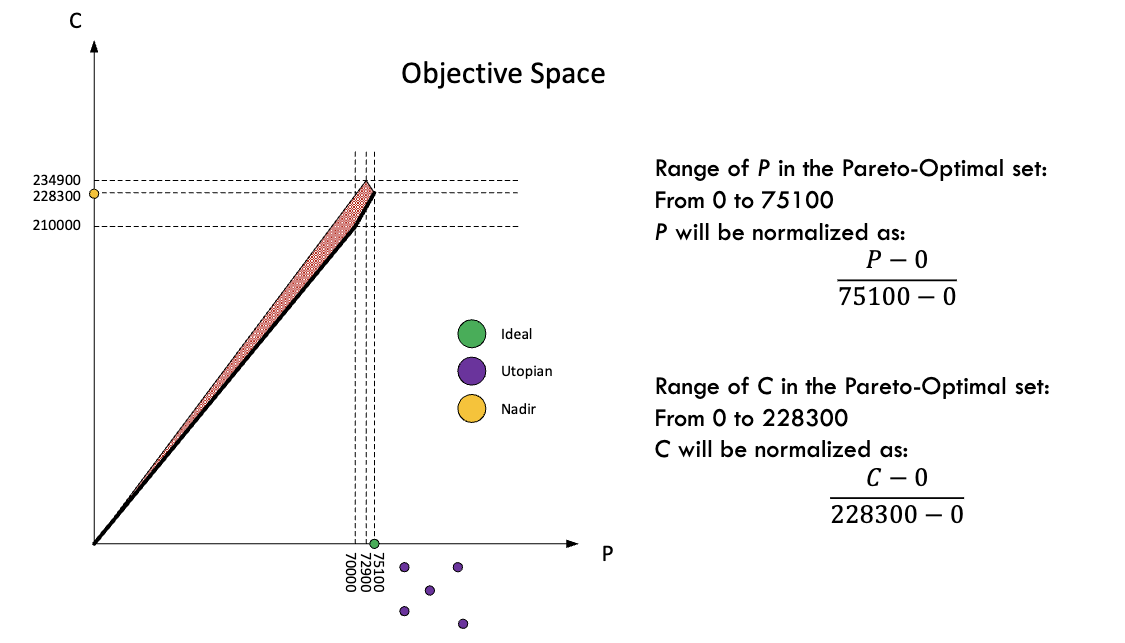
\includegraphics[width=0.8\textwidth]{2026-04-29-10-51-02.png}
\end{figure}
\newpage 
\subsection{Version 3: Maximize weighted sum of (normalized) profit and (negative) CO2 emission}
Assume profit is as important as CO2 emissions 
\begin{gather*}
    \max Z = \frac{1}{75,100}(700x_1 + 900x_2) - \frac{1}{228,300}(2100x_1 + 2900x_2)\\
    \text{s.t.}\\
    3x_1 + 4x_2 \le 324\\
    1.5x_1 + 1.2x_2 \le 150\\
    x_i \ge 0 \quad\forall i \in \{1, 2\}
\end{gather*}
(the 75k comes from the max profit, and the 228k is from the co2 emission in version 1 where we optimized for profit maximization)
\subsection{An easier way of normalizing objective functions}
Consider one of the objective functions like $F $
\begin{enumerate}
    \item Put aside all other objective functions and only keep $F $
    \item Maximize $F $ with the same set of constraints as the main problem, name it $F_\text{max} $
    \item Minimize with the same set of constraints as the main problem, name it $F_\text{min} $
    \item The normalized value of $F $ will be $\frac{F - F_\text{min}}{F_\text{max} - F_\text{min}} $

    If $F_\text{min} = 0 $, then simply you have to multiply $\frac{1}{F_\text{max}} $ to normalize it 

    In our example, you have to multiply $\frac{1}{75,100} $ into profit and $\frac{1}{234,900} $ into CO2 emissions to normalize them 
\end{enumerate}
\subsection{Version 4: maximize profit s.t. CO2 emission constraint ($\epsilon $-constrainted)}
Assume the maximum acceptable CO2 emission is 140,000 
\begin{gather*}
    \max Z = 700x_1 + 900x_2 \\
    \text{s.t.}\\
    3x_1 + 4x_2 \le 324\\
    1.5x_1 + 1.2x_2 \le 150\\
    2100x_1 + 1900x_2 \le 140000\\
    x_i \ge 0 \quad\forall i \in \{1, 2\}
\end{gather*}
\newpage 
\section{Goal programming}
Minimize the total \textbf{absolute} deviation of the objectives from the given \textbf{goals}
\begin{gather*}
    \min Z = \sum_{i = 1}^{m}w_i|f_i(x_1, x_2,\dots, x_n) - \text{Goal}_i|\\
    \text{s.t.}\\
    g_1(x_1, x_2, \dots, x_n) \le b_1\\
    g_2(x_1, x_2, \dots, x_n) \le b_2\\
    \vdots \\
    g_k(x_1, x_2, \dots, x_n) \le b_k
\end{gather*}
\subsection{Linearizing absolute deviations}
\begin{gather*}
    \min Z = \sum_{i = 1}^{m}w_i \left(F_i^{+} + F_i^-\right)\\
    \text{s.t.}\\
    F_i^{+} - F_i^- = f_i(x_1, \dots, x_n) - \text{Goal}_i\quad\forall i = 1,\dots, m \\
    F_i^{+} . F_i^- = 0\quad\forall i = 1, \dots, m\\
    F_i^{+} , F_i^- \ge 0\quad\forall i = 1, \dots, m\\
    g_j(x_1, x_2, \dots, x_n) \le b_j\quad\forall j = 1,\dots, k
\end{gather*}

\end{document}